% Author: Dominik Stolte
% Beamer presentation for DSP
% 3.1.2020

\documentclass[aspectratio=32]{beamer}
\usepackage[utf8]{inputenc}
\usepackage[T1]{fontenc} % 256 Zeichen Fonttabelle, statt 128 Zeichen
\usepackage[ngerman]{babel}
\usepackage[scaled]{helvet} 
\usepackage[font=scriptsize]{caption}
\usepackage{bookmark}
\usepackage{booktabs}
\usepackage{verbatim}
\usepackage{graphicx}
\usepackage{textpos}
\usepackage{siunitx}

\title{ELS--Rauscharme Spannungsquelle}
\author{Dominik Stolte, Dennis Henky}
\institute[{HS Mannheim}]{HS Mannheim}
\logo{
\includegraphics[height=0.8cm]{../common/hsma-logo.pdf}\vspace{235pt}}
\date{\today}
\useoutertheme{infolines}

\begin{document} 
\setbeamertemplate{itemize items}[circle]
\setbeamertemplate{navigation symbols}{}

\begin{frame}
  \titlepage{}
\end{frame}

\begin{frame}
  \frametitle{Inhalt}
  \begin{itemize}
    \item Problemstellung
    \item Schaltungssynthese
    \item Auswertung
    \item Fazit
  \end{itemize}
\end{frame}

%------------------------------------------------------------------------------
\section{Problemstellung}
{
  \logo{}
  \setbeamercolor{background canvas}{bg=black!90}
  \setbeamercolor{normal text}{fg=white}
  \setbeamertemplate{footline}{}
  \usebeamercolor*{normal text}
  \begin{frame}
    \centering
    \Large{Problemstellung}
  \end{frame}
}

\begin{frame}
  \frametitle{Problemstellung}
  \centering
  %\includegraphics[width=0.5\textwidth]{bilder/RC-tiefpass.pdf}
  \begin{itemize}
    \item Rauscharme DC Spannungserzeugung
    \item Kleine konstante Lasten
    \item Geringe PSRR notwendig
  \end{itemize}
\end{frame}

\begin{frame}
  \frametitle{Rauschen}
  \centering
  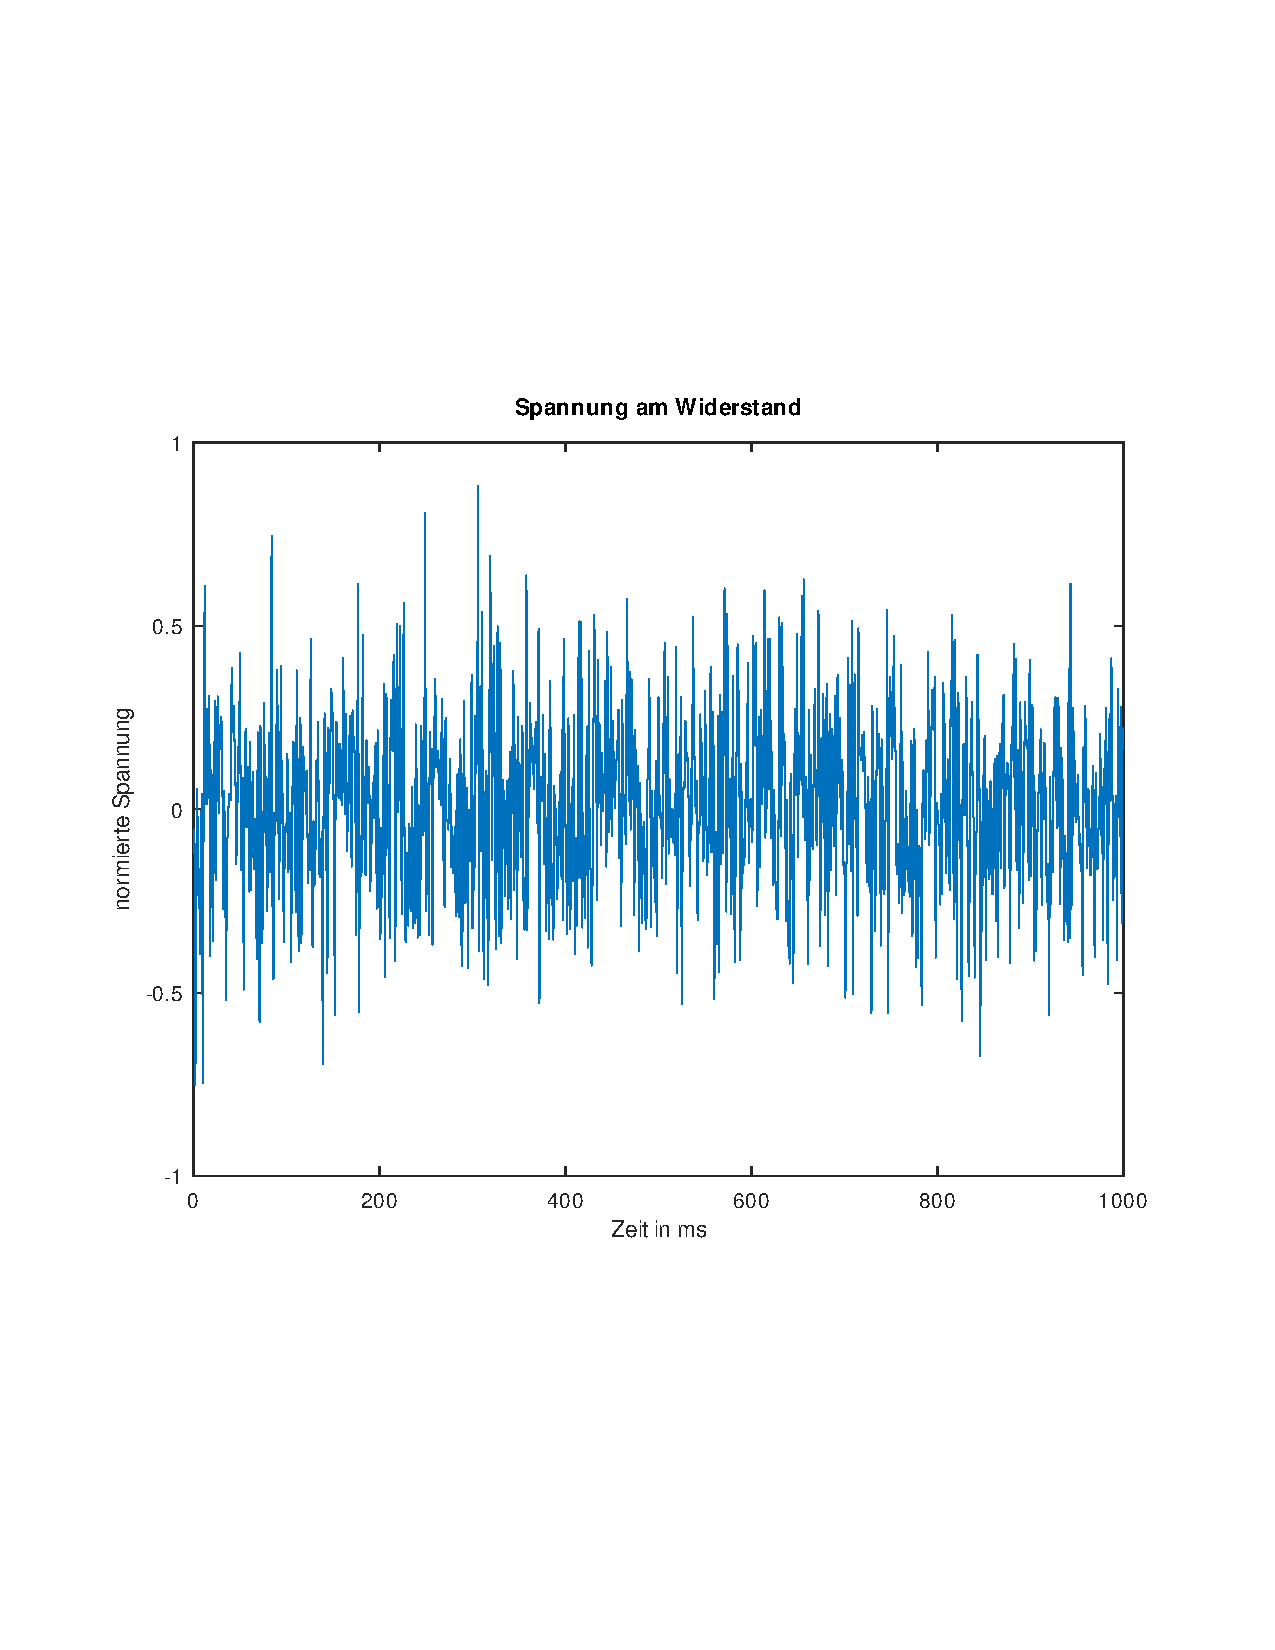
\includegraphics[width=0.5\textwidth]{../common/Simulation/rauschen/spannung.pdf}
  \begin{itemize}
    \item Zufällige Werte zu jedem Tastzeitpunkt
    \item Nur statistisch beschreibbar
  \end{itemize}
\end{frame}

\begin{frame}
  \frametitle{Rauschquellen}
  \centering
  \begin{itemize}
    \item Transistoren 
    \item Widerstände
    \item leitungsgebunden/eingestrahlt
  \end{itemize}
\end{frame}

\begin{frame}
  \frametitle{Rauschformen}
  \begin{itemize}
    \item Widerstandsrauschen (weiß)
    \item $1/f$ Rauschen (rosa)
    \item $1/f^2$ Rauschen   
  \end{itemize}
\end{frame}

\begin{frame}
  \frametitle{Rauschformen}
  \centering
  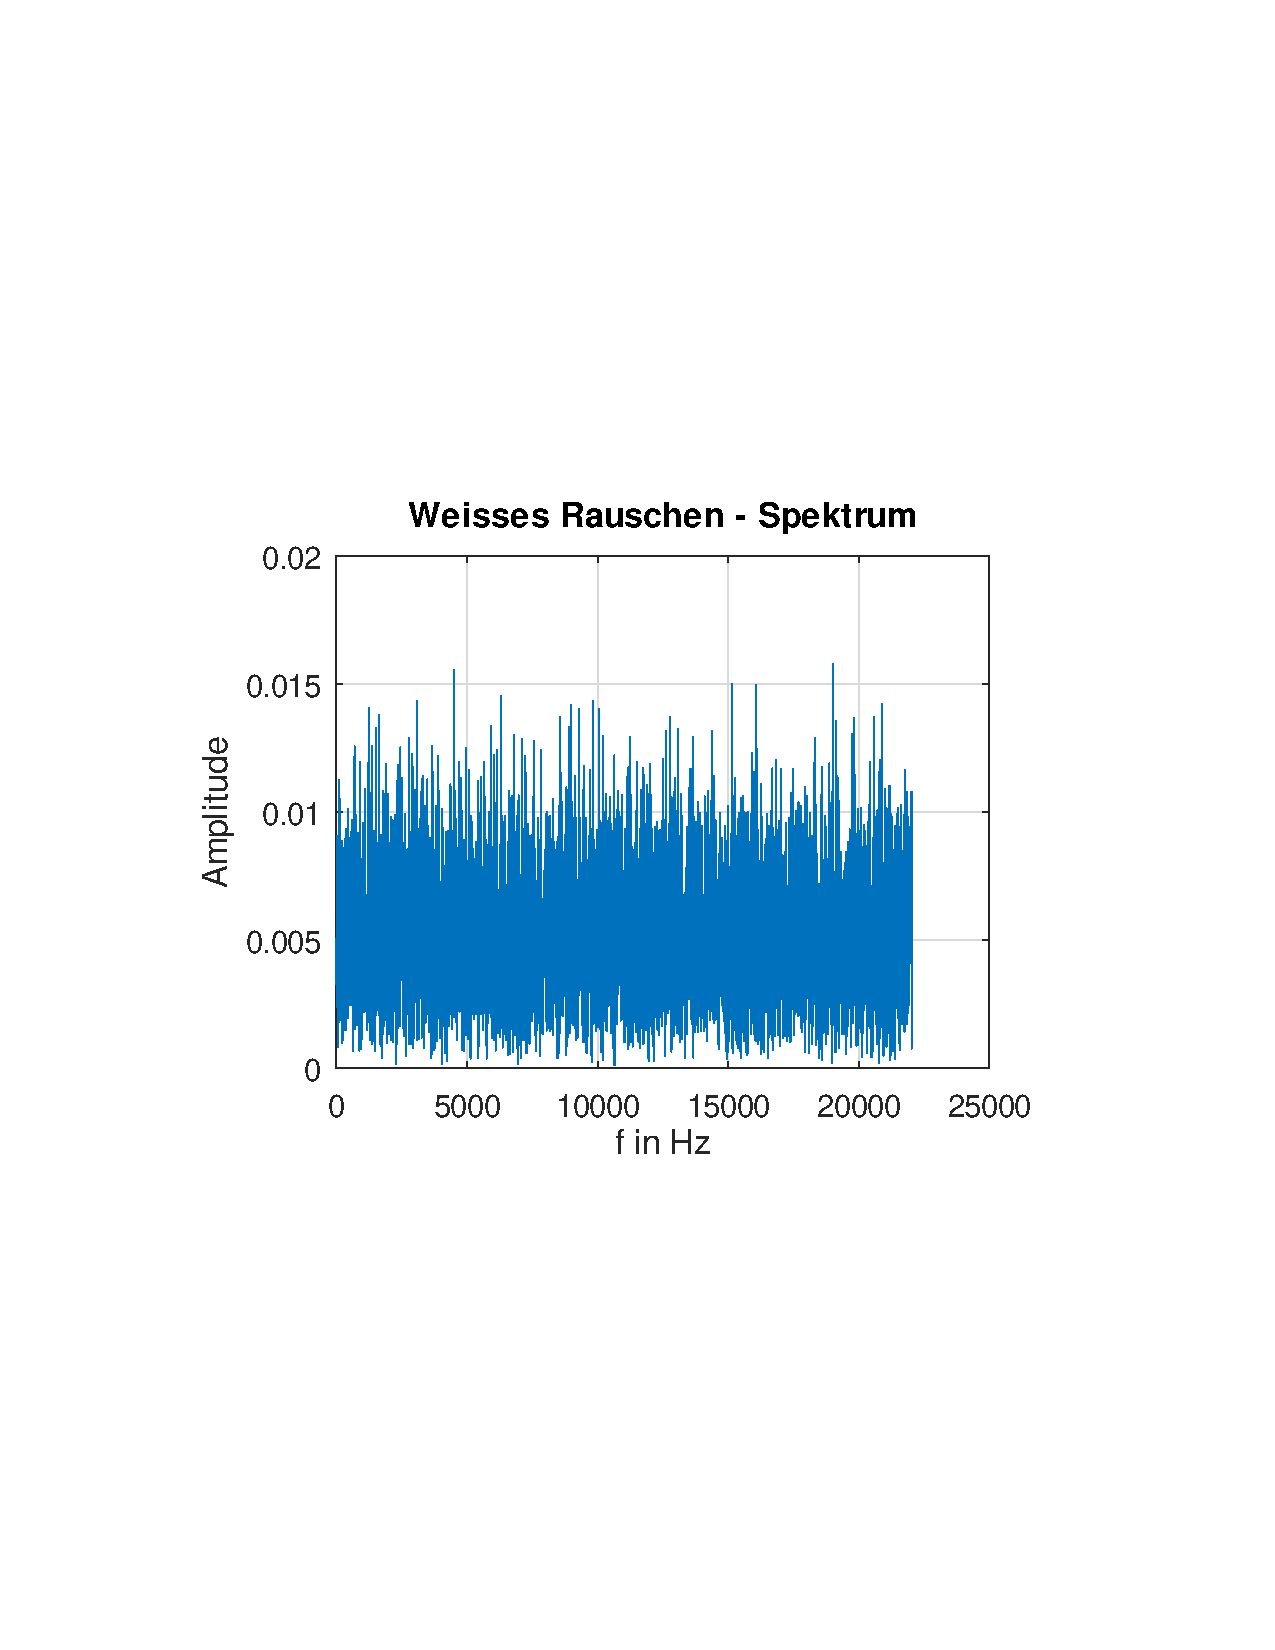
\includegraphics[width=0.45\textwidth]{../common/Simulation/audioinput/white-spkt.pdf}
  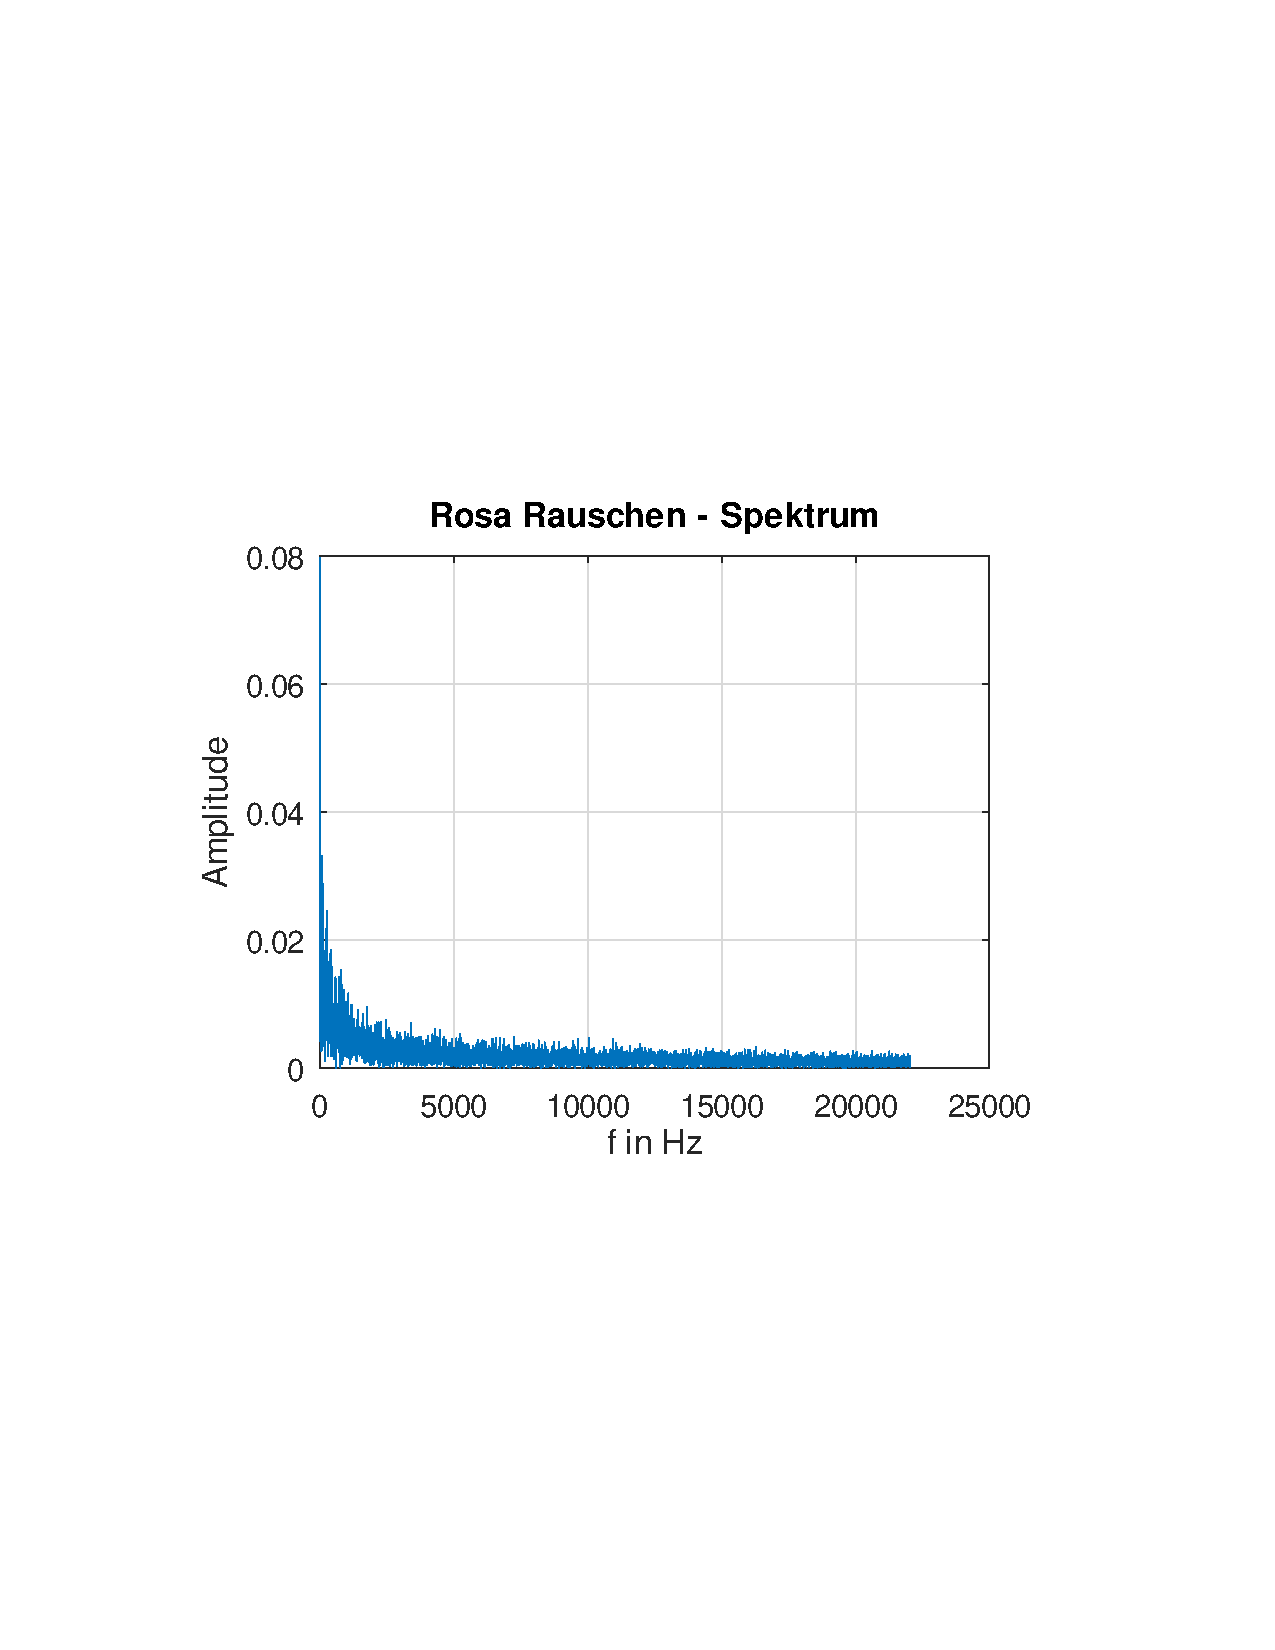
\includegraphics[width=0.45\textwidth]{../common/Simulation/audioinput/pink-spkt.pdf}
\end{frame} 

\begin{frame}
  \frametitle{Erzeugung von DC Spannungen aus dem Netz}
  \begin{itemize}
    \item Linearregler 
    \begin{itemize}
      \item integriert
      \item Operationsverstärker
      \item diskret
    \end{itemize}
    \item Schaltregler
  \end{itemize}
\end{frame}

%------------------------------------------------------------------------------
\section{Schaltungssynthese}
{
  \logo{}
  \setbeamercolor{background canvas}{bg=black!90}
  \setbeamercolor{normal text}{fg=white}
  \setbeamertemplate{footline}{}
  \usebeamercolor*{normal text}
  \begin{frame}
    \centering
    \Large{Schaltungssynthese}
  \end{frame}
}

\begin{frame}
  \frametitle{Feedbackspannungsteiler}
  \centering
  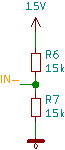
\includegraphics[height=3cm]{../common/Simulation/feedbackteiler.pdf}
  \begin{itemize}
    \item Teilt die Ausgangsspannung herunter
    \item Zielspannung $\frac{1}{2}U_{\rm out}$ 
    \item Teilung notwendig $\rightarrow$ vgl. R2R-OP
  \end{itemize}
\end{frame}

\begin{frame}
  \frametitle{Referenzspannungsquelle}
  \centering
  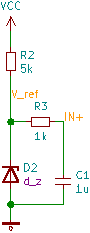
\includegraphics[height=3cm]{../common/Simulation/ref.pdf}
  \begin{itemize}
    \item Stellt stabile Referenz zur Verfügung - wenig belastbar
    \item D2 - Referenzspannung (7,5 V)
    \item R2 - Strombegrenzung für Diode
    \item R3/C1 - Tiefpass (Rauschen der Diode)
  \end{itemize}
\end{frame}

\begin{frame}
  \frametitle{Differenzverstärker}
  \centering
  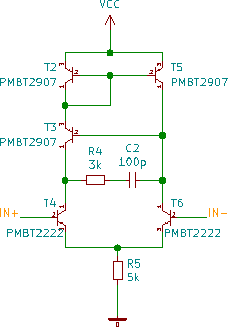
\includegraphics[width=0.2\textwidth]{../common/Simulation/diffamp.pdf}
  \begin{itemize}
    \item Herzstück der Schaltung
    \item T2/T3/T5 - Stromspiegel
    \item T4/T6 Eingangstransistoren
    \item R5 Tail ``Stromquelle''
    \item R4/C2 Kompensation
  \end{itemize}
\end{frame}

\begin{frame}
  \frametitle{Ausgangsverstärker}
  \centering
  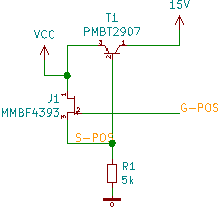
\includegraphics[height=0.4\textheight]{../common/Simulation/out.pdf}
  \begin{itemize}
    \item Stellglied des Spannungsreglers
    \item J1 - J-Fet (rauscharmer invertierender) Verstärker
    \item T1 - ``Leistungs''-Transistor
    \item R1 - Pulldownresistor und Verstärkung
  \end{itemize}
\end{frame}

%------------------------------------------------------------------------------
\section{Auswertung}
{
  \logo{}
  \setbeamercolor{background canvas}{bg=black!90}
  \setbeamercolor{normal text}{fg=white}
  \setbeamertemplate{footline}{}
  \usebeamercolor*{normal text}
  \begin{frame}
    \centering
    \Large{Auswertung}
  \end{frame}
}

\begin{frame}
  \frametitle{DC Spannungsverlauf}
  \centering
  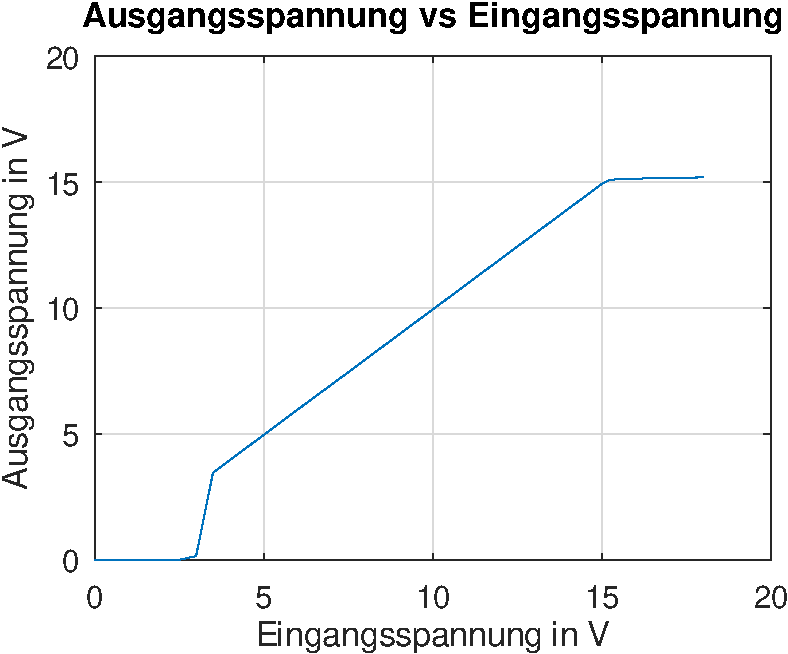
\includegraphics[height=0.5\textheight]{../common/messungen/in_vs_out.pdf}
  \begin{itemize}
    \item Der Regler regelt!
    \item Spannung am Ausgang nicht mehr proportional zur Eingangsspannung
  \end{itemize}
\end{frame}

\begin{frame}
  \frametitle{Rauschen}
  \centering
  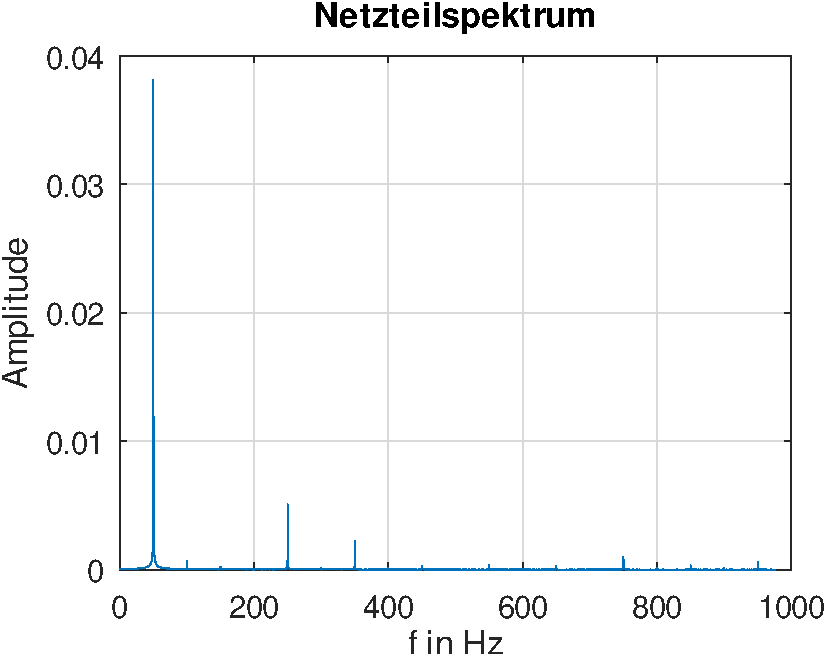
\includegraphics[width=0.3\textwidth]{../common/messungen/netzteilspektrum.pdf}
  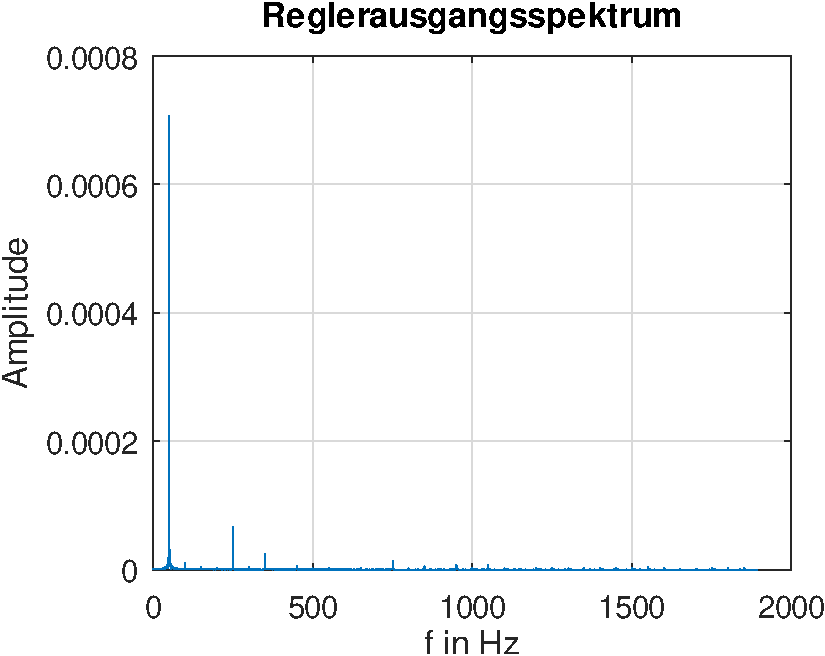
\includegraphics[width=0.3\textwidth]{../common/messungen/reglerspektrum.pdf}
  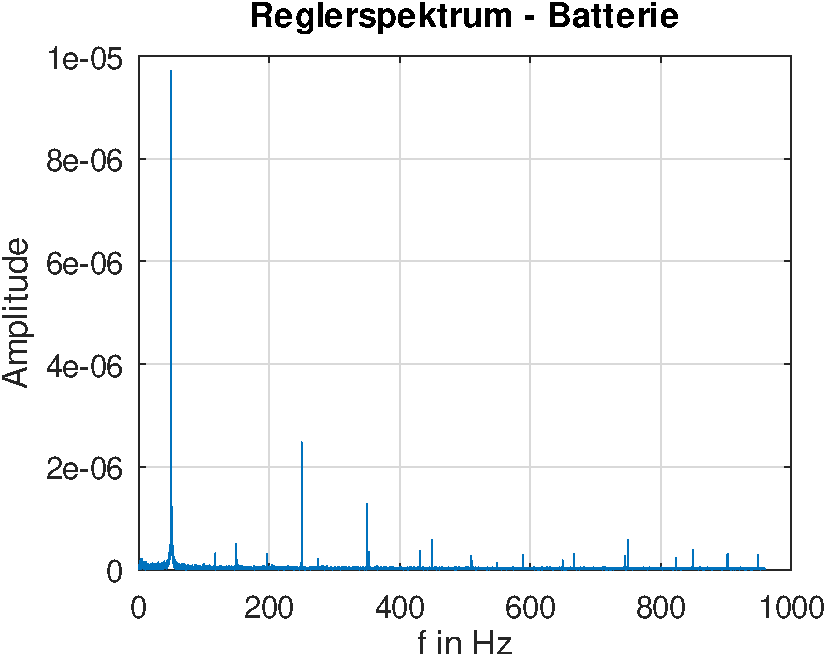
\includegraphics[width=0.3\textwidth]{../common/messungen/regler-spkt-batt.pdf}
\end{frame}


%------------------------------------------------------------------------------
\section{Fazit}
{
  \logo{}
  \setbeamercolor{background canvas}{bg=black!90}
  \setbeamercolor{normal text}{fg=white}
  \setbeamertemplate{footline}{}
  \usebeamercolor*{normal text}
  \begin{frame}
    \centering
    \Large{Fazit}
  \end{frame}
}

\begin{frame}
  \frametitle{Fazit}
  \centering
  %\includegraphics[width=0.5\textwidth]{bilder/RC-tiefpass.pdf}
  \begin{itemize}
    \item Linearregler erfolgreich gebaut
    \item Optimierungen möglich - nur einfache Bauelemente verwendet
    \item Rauschmessung äußerst schwierig. 
    50 Hz selbst bei Batteriebetrieb messbar. 
  \end{itemize}
\end{frame}

\begin{frame}
  \frametitle{Outtakes}
  \centering
  %\includegraphics[width=0.5\textwidth]{bilder/RC-tiefpass.pdf}
  \begin{itemize}
    \item Transistoren haben Beinchen
    \item Beinchen sollte man nicht vertauschen ;)
  \end{itemize}
\end{frame}

\section{Fin}
{
  \logo{}
  \setbeamercolor{background canvas}{bg=black!90}
  \setbeamercolor{normal text}{fg=white}
  \setbeamertemplate{footline}{}
  \usebeamercolor*{normal text}
  \begin{frame}
    \centering
    \Large{Ende -- Fragen}
  \end{frame}
}

\end{document}